
در این قسمت تمام عملیات‌های پردازش درخواست‌ها شامل ثبت، ویرایش و ... کنترل می‌شوند.

\begin{figure}[H]
	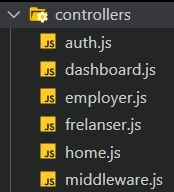
\includegraphics[width=.3\textwidth]{Folders-Files/controllers/controllers.png}
	\centering
	\caption{ساختار پوشه کنترل}
	\label{fig:folder:controllers}
\end{figure}

\subsection{فایل middleware}
در این فایل به میان‌افزارهای کنترل‌ مانند کنترل سطح دسترسی کاربر، کنترل ورود کاربر و ... پرداخته شده است.
\begin{figure}[H]
	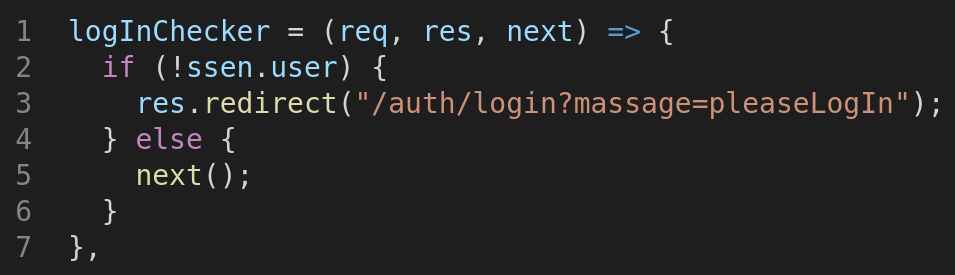
\includegraphics[width=.6\textwidth]{Folders-Files/controllers/controllers-middleware.png}
	\centering
	\caption{ساختار فایل middleware}
	\label{fig:file:controllers:middleware}
\end{figure}

\paragraph{\rl{logInChecker}:}
اعتبارسنجی ورود کاربر به سایت.
\\
\textbf{توضیحات}
\hr
\begin{flushleft}
	\framebox[.9\textwidth][l]{
		\lr{
			\textcolor{type}{void}
			\textcolor{func}{logInChecker}
			\textcolor{symb}{(}
			\textcolor{type}{object}
			\textcolor{arg}{request}
			\textcolor{symb}{,}
			\textcolor{type}{object}
			\textcolor{arg}{response}
			\textcolor{symb}{,}
			\textcolor{type}{object}
			\textcolor{arg}{next}
			\textcolor{symb}{);}
		}
	}
\end{flushleft}
بررسی طلاعات کاربری و اعتبار زمانی.
\\
\textbf{پارامترها}
\hr \\[10pt]
\begin{tabular}{|m{4cm}|m{3cm}|m{10cm}|}
	\hline
	\multicolumn{1}{|c}{پارامتر}
	&
	\multicolumn{1}{|c}{نوع}
	&
	\multicolumn{1}{|c|}{توضیحات}
	\\
	\hline
	\multicolumn{1}{|c}{request}
	&
	\multicolumn{1}{|c|}{object}
	&
	نمایانگر درخواست HTTP و دارای خصوصیاتی برای درخواست رشته پرس‌و‌جو، پارامترها ، بدنه ، هدرهای HTTP و غیره است.
	در این اسناد و طبق قرارداد ، از این شی همیشه به عنوان req یاد می شود (و پاسخ HTTP res است).
	\\
	\hline
	\multicolumn{1}{|c}{response}
	&
	\multicolumn{1}{|c|}{object}
	&
	نمایانگر پاسخ HTTP که برنامه Express با دریافت درخواست HTTP ارسال می کند.
	در این اسناد و طبق قرارداد ، از شی همیشه به عنوان res یاد می شود (و درخواست HTTP req است).
	\\
	\hline
	\multicolumn{1}{|c}{next}
	&
	\multicolumn{1}{|c|}{object}
	&
عملکرد میان‌افزار بعدی را نشان می دهد.
	\\
	\hline
\end{tabular}
\\[10pt]
\textbf{خروجی}
\hr \\
در صورتی که کاربر به سایت وارد شده باشد یا مهلت زمانی ورود کاربر به پایان نرسیده باشد برنامه ادامه می‌یابد، در غیر این صورت به صفحه ورود به سایت هدایت می‌شود.

\subsection{فایل auth}
در این فایل به کنترل عملیات‌های احرازهویت پرداخته شده است.
\begin{figure}[H]
	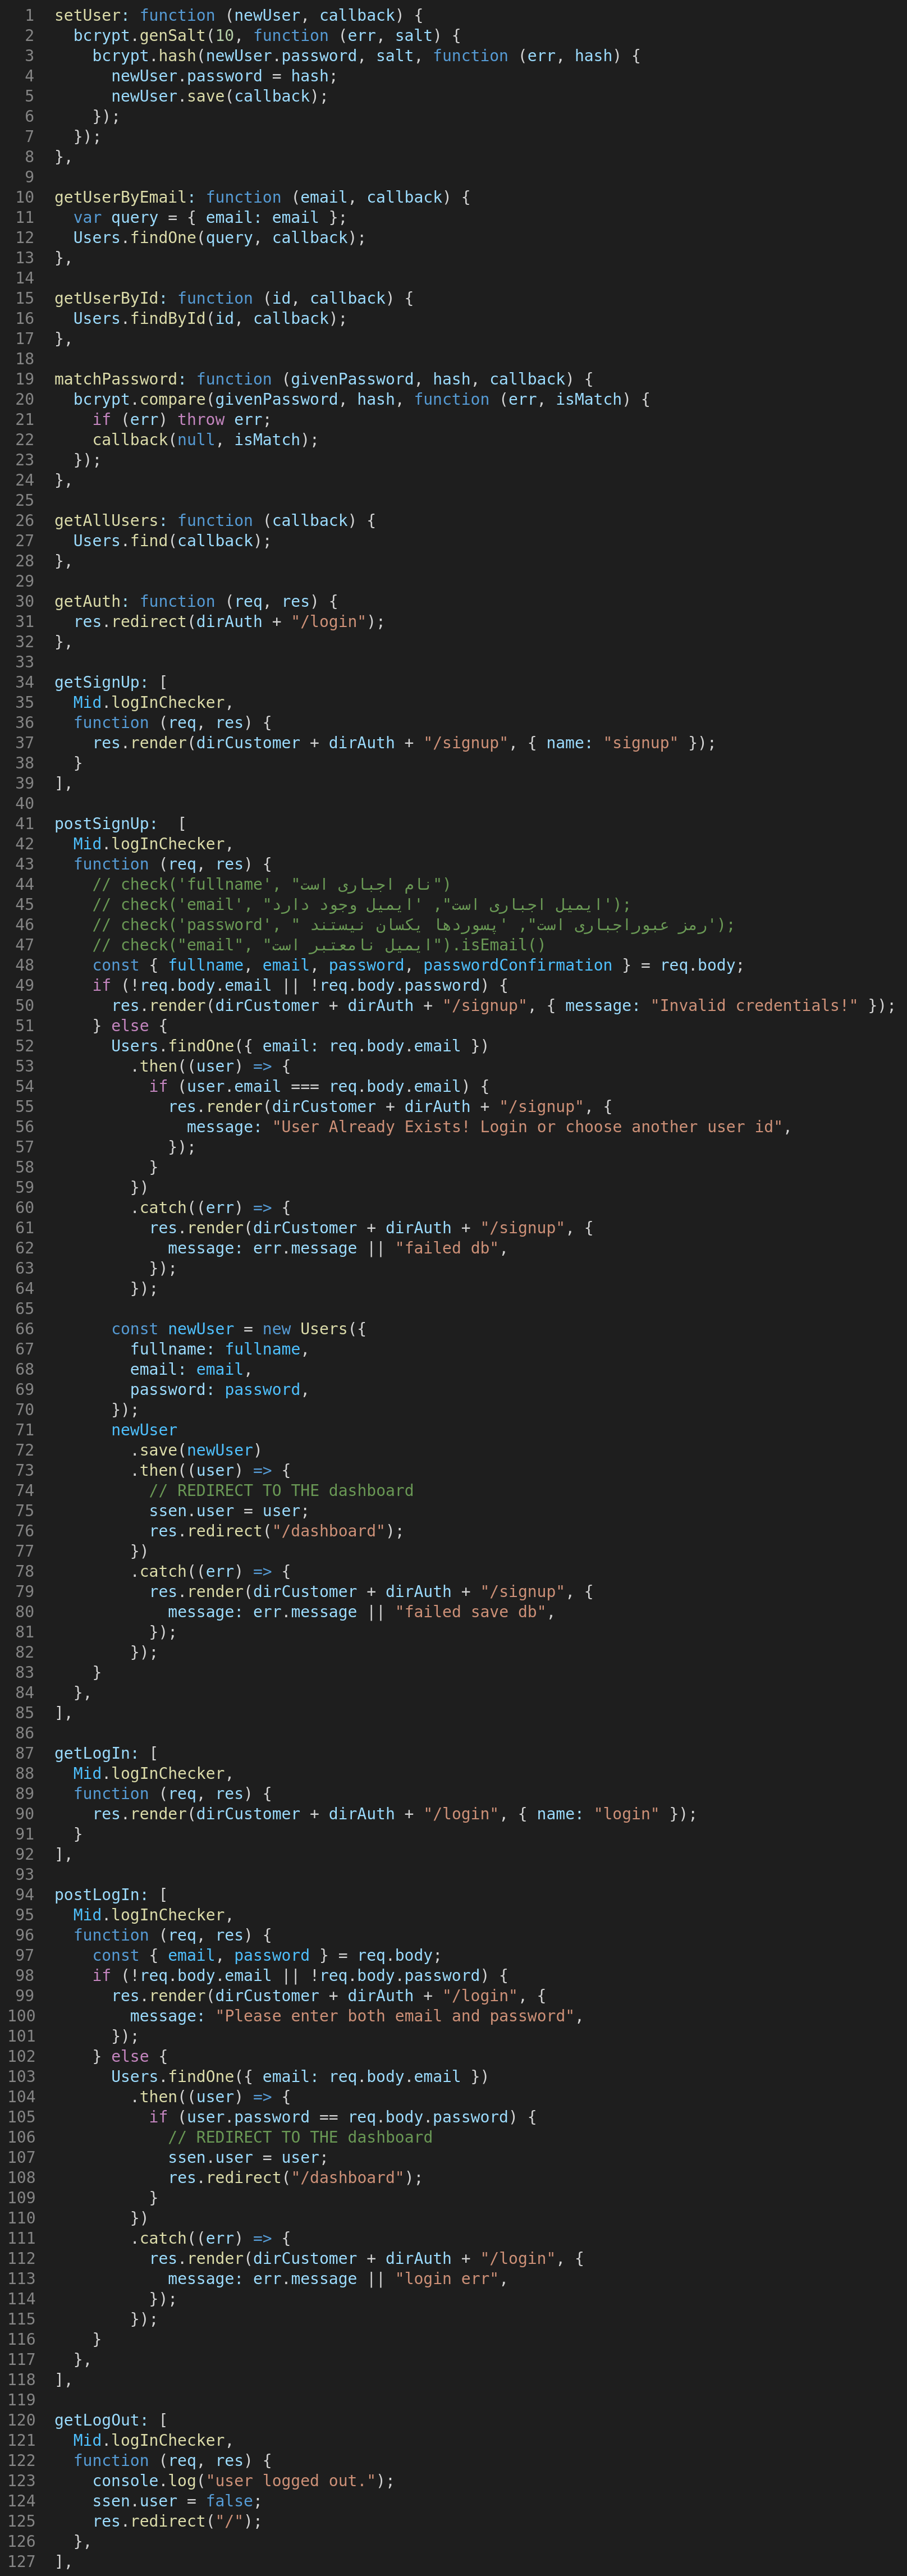
\includegraphics[width=.6\textwidth]{Folders-Files/controllers/controllers-auth.png}
	\centering
	\caption{ساختار فایل auth}
	\label{fig:file:controllers:auth}
\end{figure}

\paragraph{\rl{setUser}:}
ثبت اطلاعات کاربر.
\\
\textbf{توضیحات}
\hr
\begin{flushleft}
	\framebox[.9\textwidth][l]{
		\lr{
			\textcolor{type}{void}
			\textcolor{func}{setUser}
			\textcolor{symb}{(}
			\textcolor{type}{object}
			\textcolor{arg}{newUser}
			\textcolor{symb}{,}
			\textcolor{type}{object}
			\textcolor{arg}{callback}
			\textcolor{symb}{);}
		}
	}
\end{flushleft}
ثبت طلاعات کاربر در بانک اطلاعات.
\\
\textbf{پارامترها}
\hr \\[10pt]
\begin{tabular}{|m{4cm}|m{3cm}|m{10cm}|}
	\hline
	\multicolumn{1}{|c}{پارامتر}
	&
	\multicolumn{1}{|c}{نوع}
	&
	\multicolumn{1}{|c|}{توضیحات}
	\\
	\hline
	\multicolumn{1}{|c}{newUser}
	&
	\multicolumn{1}{|c|}{object}
	&
0
	\\
	\hline
	\multicolumn{1}{|c}{callback}
	&
	\multicolumn{1}{|c|}{object}
	&
0
	\\
	\hline
\end{tabular}
\\[10pt]
\textbf{خروجی}
\hr \\
در صورتی که ، در غیر این صورت .


\paragraph{\rl{getUserByEmail}:}
دریافت اطلاعات کاربر با پست الکترونیک.
\\
\textbf{توضیحات}
\hr
\begin{flushleft}
	\framebox[.9\textwidth][l]{
		\lr{
			\textcolor{type}{void}
			\textcolor{func}{getUserByEmail}
			\textcolor{symb}{(}
			\textcolor{type}{string}
			\textcolor{arg}{email}
			\textcolor{symb}{,}
			\textcolor{type}{object}
			\textcolor{arg}{callback}
			\textcolor{symb}{);}
		}
	}
\end{flushleft}
دریافت طلاعات کاربر از بانک اطلاعات توسط پست الکترونیک.
\\
\textbf{پارامترها}
\hr \\[10pt]
\begin{tabular}{|m{4cm}|m{3cm}|m{10cm}|}
	\hline
	\multicolumn{1}{|c}{پارامتر}
	&
	\multicolumn{1}{|c}{نوع}
	&
	\multicolumn{1}{|c|}{توضیحات}
	\\
	\hline
	\multicolumn{1}{|c}{email}
	&
	\multicolumn{1}{|c|}{string}
	&
	0
	\\
	\hline
	\multicolumn{1}{|c}{callback}
	&
	\multicolumn{1}{|c|}{object}
	&
	0
	\\
	\hline
\end{tabular}
\\[10pt]
\textbf{خروجی}
\hr \\
در صورتی که ، در غیر این صورت .


\paragraph{\rl{getUserById}:}
دریافت اطلاعات کاربر با ID.
\\
\textbf{توضیحات}
\hr
\begin{flushleft}
	\framebox[.9\textwidth][l]{
		\lr{
			\textcolor{type}{void}
			\textcolor{func}{getUserById}
			\textcolor{symb}{(}
			\textcolor{type}{int}
			\textcolor{arg}{id}
			\textcolor{symb}{,}
			\textcolor{type}{object}
			\textcolor{arg}{callback}
			\textcolor{symb}{);}
		}
	}
\end{flushleft}
دریافت طلاعات کاربر از بانک اطلاعات توسط ID.
\\
\textbf{پارامترها}
\hr \\[10pt]
\begin{tabular}{|m{4cm}|m{3cm}|m{10cm}|}
	\hline
	\multicolumn{1}{|c}{پارامتر}
	&
	\multicolumn{1}{|c}{نوع}
	&
	\multicolumn{1}{|c|}{توضیحات}
	\\
	\hline
	\multicolumn{1}{|c}{id}
	&
	\multicolumn{1}{|c|}{int}
	&
	0
	\\
	\hline
	\multicolumn{1}{|c}{callback}
	&
	\multicolumn{1}{|c|}{object}
	&
	0
	\\
	\hline
\end{tabular}
\\[10pt]
\textbf{خروجی}
\hr \\
در صورتی که ، در غیر این صورت .


\subsection{فایل employer}
در این فایل به کنترل تمام عملیات‌های داشبورد کارفرما پرداخته شده است.
\begin{figure}[H]
	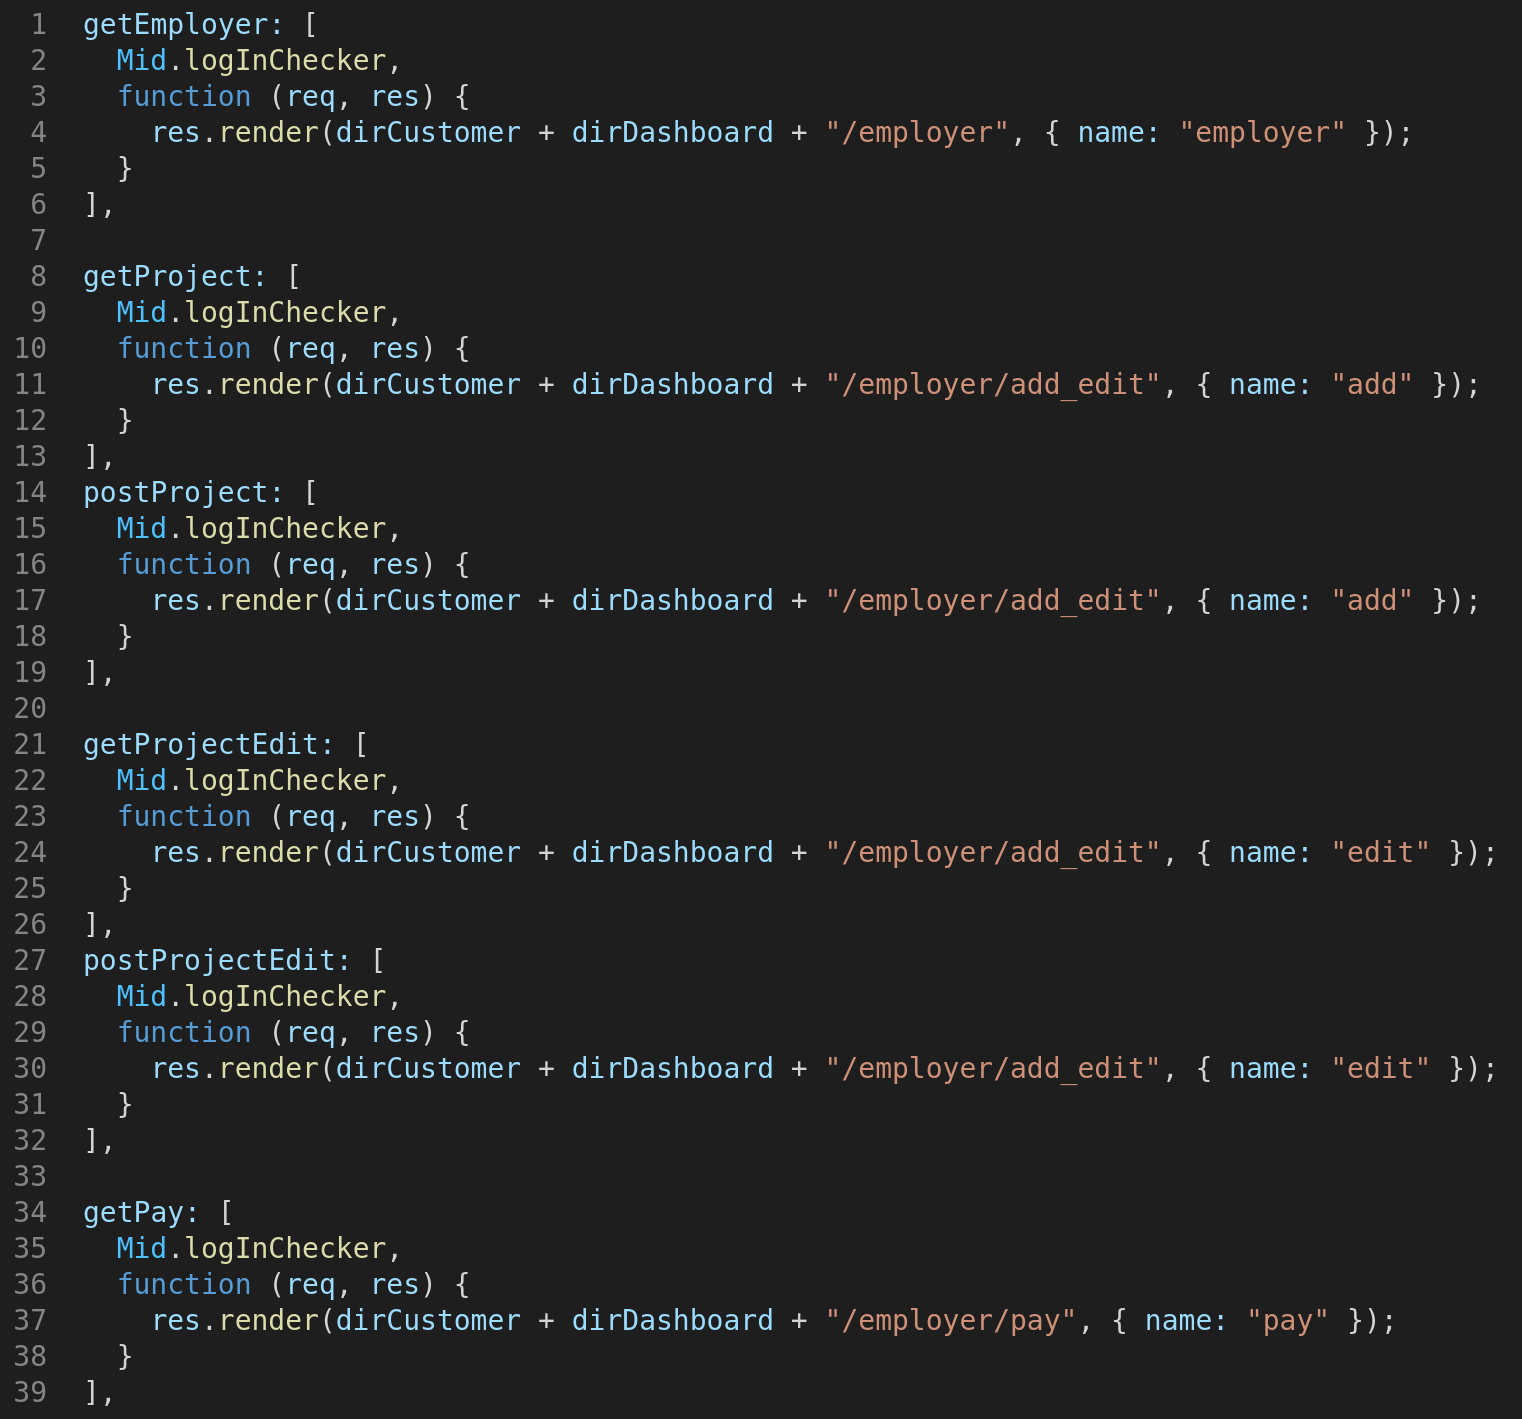
\includegraphics[width=.6\textwidth]{Folders-Files/controllers/controllers-employer.png}
	\centering
	\caption{ساختار فایل employer}
	\label{fig:file:controllers:employer}
\end{figure}

\subsection{فایل frelanser}
در این فایل به کنترل تمام عملیات‌های داشبورد فریلنسر پرداخته شده است.
\begin{figure}[H]
	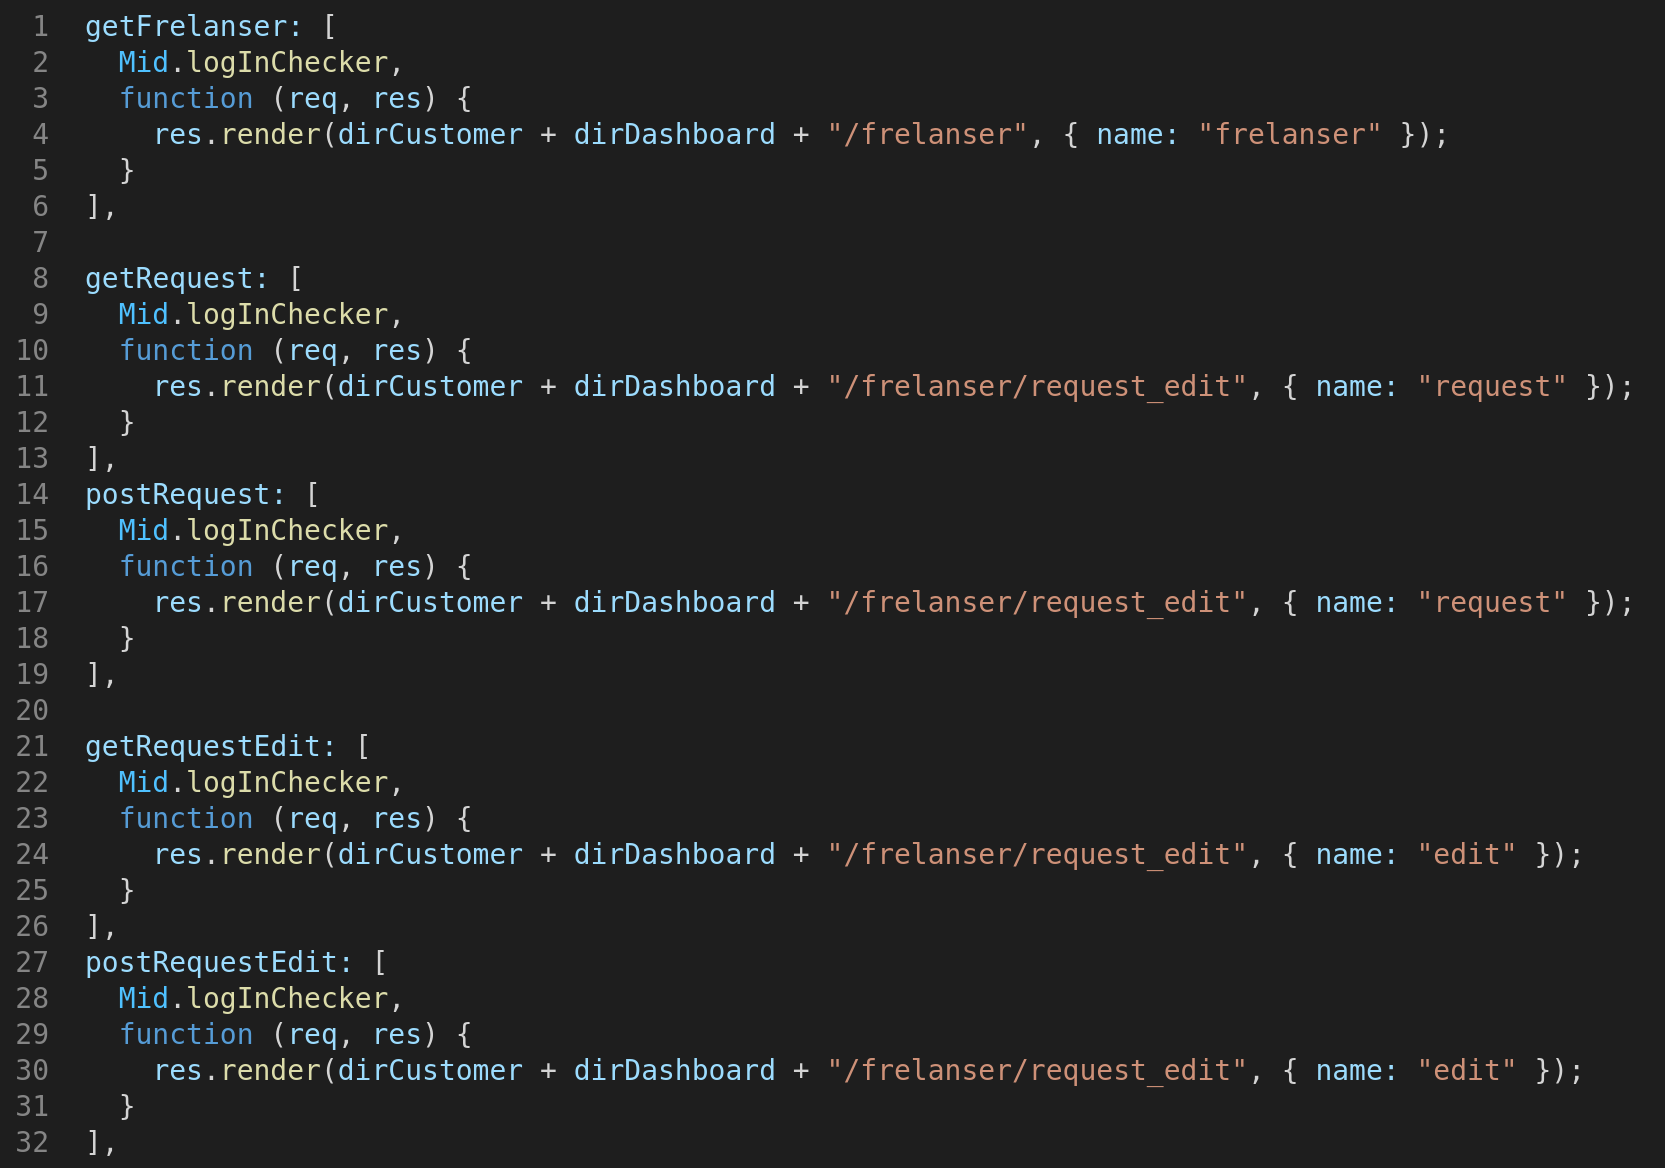
\includegraphics[width=.6\textwidth]{Folders-Files/controllers/controllers-frelanser.png}
	\centering
	\caption{ساختار فایل frelanser}
	\label{fig:file:controllers:frelanser}
\end{figure}
